\section{Experiments}

\subsection{Experiment Setup}





\paragraph{Data}
We use DBpedia~\cite{auer2007dbpedia}, a large-scale knowledge graph constructed from Wikipedia. 
We report the statistics of the DBpedia knowledge graph in Table \ref{tab:dbpedia_stat}.  Note that there are ``dummy'' entities in DBpedia that represent a fact that is only true on a specific time period. An example is \url{https://dbpedia.org/page/Kathy\_Greenlee\_\_Tenure\_\_1}. For simplicity, we remove these dummy entities and triples related from the knowledge graph. We refer to the remaining triples as the DBpedia knowledge graph. The DBpedia knowledge graph contains 4,928,232 entities, 633 relations, and 16,915,848 triples. The average node degree of the knowledge graph is 6.80, and the density of the knowledge graph is $7.18\times 10^{-7}$. 

\begin{table}[t]
\centering\small
\begin{tabular}{c|c|c|c|c}
\toprule
\textbf{\#Entities} & \textbf{\#Relations} & \textbf{\#Triples} &  \textbf{Avg. degree} & \textbf{Density} \\ \midrule
4,928,232 & 633 & 16,915,848 & 6.80 & $7.18\times 10^{-7}$ \\ \bottomrule
\end{tabular}
\vspace{-2mm}
\caption{Statistics of the DBpedia knowledge graph.}
\label{tab:dbpedia_stat}
\vspace{-5mm}
\end{table}




 
   

\paragraph{LLMs}
In this paper, we evaluate the Meta LLaMA 2 family~\cite{touvron2023llama}, including LLaMA-2-7B, LLaMA-2-13B, and LLaMA-2-70B, and Google's Gemma~\cite{gemmateam2024gemma} including Gemma-2B and Gemma-7B. 
For each language model, we first randomly sample 2000 triples, and perform a negative sampling to obtain another 2000 negative triples. For each triple, we ask the LLM 3 times the same question, on whether the triple is true, false, or the LLM doesn't know. We use majority voting to determine the LLM's final answer. When asking, we use huggingface's pipeline with default settings and FP16 precision. 
 This is to form a labeled dataset. We randomly sample 70\% for the training set and 30\% for the validation set, then train a judge model to classify the LLM's hidden state into 3 classes: LLM correctly answering the question (True), LLM incorrectly answering the question (False), and LLM responding with I don't know (IDK). We refer to Table \ref{tab:llm_stat} for the statistics of the labeled dataset.


\paragraph{Metrics}
 For the LLM's performance, we report the estimated factuality of the LLMs on the DBpedia knowledge graph. We report the LLM's performance in terms of \textit{Truthfulness}, \textit{Informativeness}, and \textit{Correctness}. For evaluating the judge model's performance (See Appendix~\ref{app:judge_model}), we seek to maximize the similarity between the judge model's prediction and the LLM's answer. Thus, we use the common metrics Precision (P), Recall (R), and F1 score (F) to evaluate the judge model's accuracy; and the time it takes to predict to evaluate the judge model's efficiency.

\paragraph{Hyperparameter Settings}
For the judge model classifier training, we train 100 epochs with a batch size of 8. We use the Adam optimizer with a learning rate of 1e-4. We use the same settings for all the evaluated LLMs. For LLaMA 2 7B, 13B, and 70B, we use LLaMA 2 7B as the judge model's hidden state input. For Gemma 2B and 7B, we use Gemma 2B as the judge model's hidden state input.
 The judge model is trained on a server with NVIDIA A6000 GPUs.

For the training of the prompt encoder, we use the same settings for all the evaluated LLMs. To be specific, we use 20 virtual tokens, 1 transformer submodule, 12 attention heads, 12 layers, MLP as the encoder reparameterization type, 4096 as the encoder hidden size, and 2e-5 as the learning rate. We train the prompt encoder for 5 epochs with a batch size of 8. We use the Adam optimizer with a weight decay of 0.01.

 For the evaluation, we use two servers, one with NVIDIA A6000 GPUs and the other with NVIDIA A100 GPUs. For inference, we use Flash Attention 2~\cite{dao2023flashattention2} as the attention implementation, and use FP16 precision.


\subsection{LLM's Performance Analysis}\label{sub:performance_analysis}


We report the estimated factuality of the LLMs on DBpedia in Table \ref{tab:llm_stat}. 
Overall, the LLaMA-2 series shows an increase in model size up to 13B, particularly in terms of balanced \textit{truthfulness}, \textit{informativeness}, and \textit{correctness}. However, the 70B variant diverges, excelling in \textit{truthfulness} but failing to provide useful or accurate information. We will discuss this phenomenon in the detailed LLaMA analysis. 
The Gemma series struggles with \textit{truthfulness} and \textit{correctness}, despite being \textit{informative}. This might indicate that these models are better at generating detailed content but need careful consideration for tasks requiring high accuracy or reliability.
The performance of these models highlights the complex trade-offs between being \textit{truthful}, \textit{informative}, and \textit{correct}. 
We further provide a correlation analysis between the LLM's performance and the degree/popularity of the entities in the Appendix~\ref{app:correlation_analysis}.



\paragraph{LLaMA-2 Analysis}
LLaMA-2-7B shows good \textit{truthfulness} (.965) but is moderate in being \textit{informative} (.550) and \textit{correct} (.516). This suggests that while the model is generally reliable in its outputs, it may not always provide highly detailed or accurate information.
LLaMA-2-13B significantly improves across all metrics compared to LLaMA-2-7B, with very high scores in \textit{truthfulness} (.979), \textit{informativeness} (.980), and \textit{correctness} (.959). This indicates a strong overall performance, making it a very reliable and accurate model for generating information.

LLaMA-2-70B, despite its high \textit{truthfulness} (.993), scores extremely low in both \textit{informativeness} (.007) and \textit{correctness} (.006), which is puzzling. 
We hypothesize that the model may have difficulty in making a decision, and thus selecting `I don't know' as the answer. This may be related to a more clear knowledge boundary of LLMs, as larger LMs tend to give up on more questions~\cite{ren2023investigating}, meaning they have a better understanding on whether they know the answer or not. {A detailed analysis of the knowledge boundary of LLMs can be found in Appendix \ref{app:knowledge_boundary}.} This can also be confirmed by the fact that the model has the highest \textit{truthfulness} score among all models, indicating that it is more likely to provide a correct answer when it knows the answer. However, it is still important to note that a high number of `I don't know' answers may indicate the model's inability to answer factual questions. 

\paragraph{Gemma Analysis}
Gemma-2B has an exceptionally low \textit{truthfulness} score (.056) but is quite high in \textit{informativeness} (.867). Its \textit{correctness} score (.024) is also very low. This suggests that despite providing detailed responses, the model's outputs are often neither \textit{truthful} nor accurate. It might be generating detailed but misleading or incorrect information.
Gemma-7B improves on \textit{truthfulness} (.206) compared to Gemma-2B but still falls short of being considered reliable. Its \textit{informativeness} (.657) is respectable, and its \textit{correctness} (.056) remains low. Similar to Gemma-2B, while it can provide detailed responses, those are not often true or correct.






\begin{table}[t]
    \centering\small
    \begin{tabular}{l|ccc|ccc}
    \toprule
    \textbf{Model} & \textbf{True} & \textbf{False} & \textbf{IDK} & \textbf{Truthful} & \textbf{Informative} & \textbf{Correct} \\ 
    \midrule
    LLaMA-2-7B & 1901 & 1545 & 554 & 0.965 & 0.550 & 0.516 \\
    LLaMA-2-13B & 2100 & 1796 & 104 & 0.979 & 0.980 & 0.959 \\
    LLaMA-2-70B & 338 & 126 & 3536 & 0.993 & 0.007 & 0.006 \\
    Gemma-2B & 1760 & 1786 & 454 & 0.056 & 0.867 & 0.024 \\
    Gemma-7B & 1509 & 1751 & 740 & 0.206 & 0.657 & 0.056 \\
    \bottomrule
    \end{tabular}
    \caption{Statistics and performance metrics of LLMs. True, False, and IDK denote the number of labels from the LLMs in the labeled dataset. \Truthful, \Informative, and \Correct{} represent performance metrics.}
    \label{tab:llm_stat}
    \vspace{-3mm}
\end{table}


\vspace{-2mm}
\subsection{Relation Type Study}

 

\begin{figure}[t]
\centering
 
\includegraphics[width=5.5in]{submissions/Jing2024/figures/experiments/relation_analysis/legend.pdf}
\\\vspace{-6mm}
\subfloat[\textit{Averaged metrics} vs Head entity type]{
 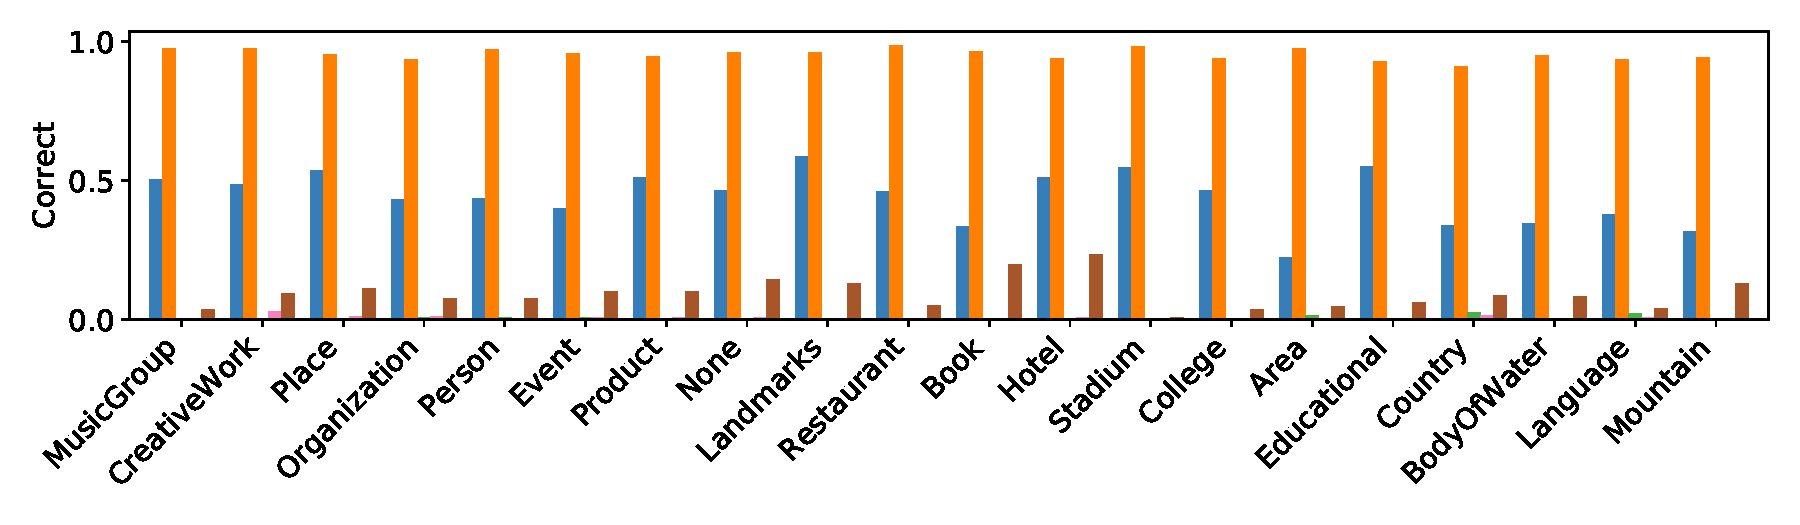
\includegraphics[width=5.5in]{submissions/Jing2024/figures/experiments/relation_analysis/correct_by_head_type.pdf}
 \label{fig:avg_by_head_type}
}\\
\vspace{-4mm}
\subfloat[\textit{Averaged metrics} vs Tail entity type]{
 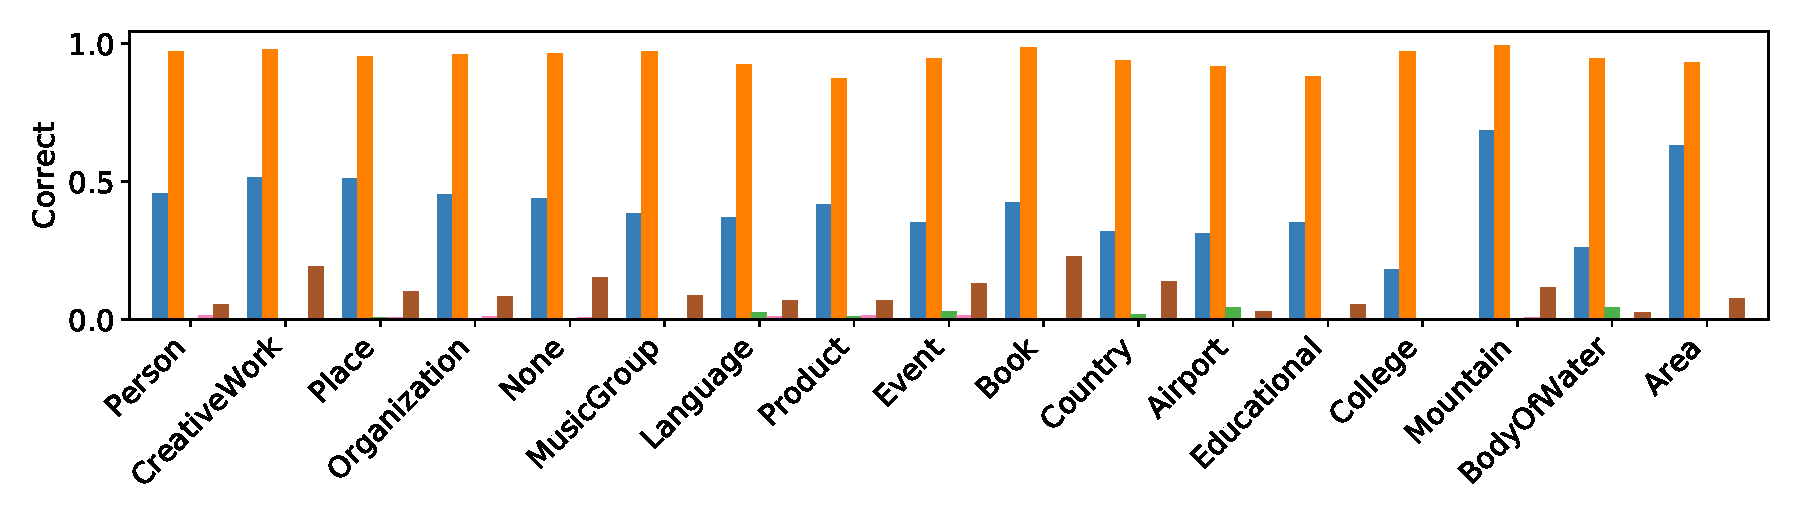
\includegraphics[width=5.5in]{submissions/Jing2024/figures/experiments/relation_analysis/correct_by_tail_type.pdf}
 \label{fig:avg_by_tail_type}
}
\vspace{-4mm}
\caption{The LLM's {\it averaged metrics} with respect to head entity types and tail entity types}
\vspace{-3mm}
\label{fig:avg_by_type}
\end{figure}


\label{exp:relation_type_study} 
There are more than 600 different relation types in the DBpedia knowledge graph, and each relation type has different characteristics. It is unclear if we directly compare the performance of the LLMs on different relation types.
Thus, to gain a better understanding of the LLM's performance, we first analyze the LLM's performance with respect to relation types. In DBpedia, most entities are associated with a \url{https://schema.org/} type. Thus, we can categorize the relations into different types by the triples they belong to. We denote a relation's head/tail entity type as the most frequent schema type of the head/tail entity of the triples associated with the relation.
 For example, the relation \texttt{birthPlace} is associated with triples like \texttt{(Barack Obama, birthPlace, Hawaii)}, and the head entity \texttt{Barack Obama} is associated with the schema type \texttt{Person}, and the tail entity \texttt{Hawaii} is associated with the schema type \texttt{Place}. Then, the relation's head entity type is \texttt{Person}, and tail entity type is \texttt{Place}.
 We then analyze the LLM's performance with respect to these relation types. We report the performance of the LLMs on different relation types, by taking the average of the 3 metrics, \textit{correctness}, \textit{truthfulness}, and \textit{informativeness}, for each relation type. We present the results in Figure~\ref{fig:avg_by_type}. Here, ``None'' refers to entities not linked to a schema type. We also present a detailed analysis of the LLM's performance with respect to head and tail entity types in Appendix~\ref{app:relation_type_study}.
We can observe variability in model performance across relation types, such as ``MusicGroup" and ``CreativeWork" achieving high scores while ``Area" and "Mountain" face lower performance, highlighting the diverse challenges in modeling different kinds of information. These performance differences suggest that the effectiveness of LLMs in handling structured knowledge heavily depends on the nature of the relations being modeled.













